\subsubsection{Accuracy} 
To check the accuracy of the methods, we compare the voltage output of the integrated methods with the output of the separated methods. We solve the transmission network separately using NR-power and we solve the distribution network separately using NR-TCIM. The distribution domain in the integrated network has no reference bus anymore. In order to compare the voltage profile of this part, we scale the values accordingly. 
We know that the voltage is given by: \begin{equation}
V_p=|V|_p\exp{(\iota\delta_{V_p}-\phi)},\quad p\in\{a,b,c\},
\end{equation}
where $|V|$ and $\delta$ are set to $|V|=1.0$ pu and $\delta=0$ at the reference bus. We can compare the voltage of the distribution domain to the voltage of the separated domain after scaling. We divide the voltage magnitude of the distribution domain, buses $i=1,...,N_D$, by the voltage magnitude of the distribution connection bus: 
\begin{equation}
|V|_{i,{D_{new}}} = \frac{|V|_{i,{D_{uns}}}}{|V|_{ref,{D_{uns}}}},\quad i=1,..,N_D.
\label{eq:ViDnew}
\end{equation}
The subscript $uns$ represents the unscaled values and $new$ represents the scaled values. \newline 
The voltage angle represents the phase-shift in relation to the phase of the reference bus. In order to compare the integrated output of the voltage angle with the separated output, we subtract the phase-angle of the former reference bus from all the buses $i=1,..,N_D$: 
\begin{equation}
\delta_{i,{D_{new}}} ={\delta_{i,{D_{uns}}}}-{\delta_{ref,{D_{uns}}}},\quad i=1,..,D_N.
\label{eq:dViDnew}
\end{equation}
Note that we need to apply \eqref{eq:ViDnew} and \eqref{eq:dViDnew} to all the three phases separately. \newline\newline
We compare the voltage magnitudes and angles of the integrated network, including the scaled distribution domain, with the magnitudes angles of the separate domains. We take the infinity norm of the relative difference between the voltages: 
\begin{equation}
\mbox{rel. error of } |V|_p = \left|\frac{|V|^*_p - |V|^o_p}{|V|^o_p}\right|_\infty,\quad p\in\{a,b,c\},
\label{eq:norm|V|}
\end{equation}
where the asterisk $*$ marks the outcome of separated networks, and the superscript $o$ the output of separated networks (o=original). We do this in a similar manner for the voltage angle: 
\begin{equation}
\mbox{rel. error of } \delta_p = \left|\frac{\delta^*_p - \delta^o_p}{\delta^o_p}\right|_\infty,\quad p\in\{a,b,c\},
\label{eq:normdelta}
\end{equation}
We have given the relative errors of the voltage magnitude and angle of the three phases for all the test cases in table \ref{tab:relerror}. 

\begin{table}[h]
\renewcommand{\arraystretch}{1.3}
\centering
\caption{Relative error of the voltage magnitude and angle of the three phases for all the integration methods. }\label{tab:relerror}
\begin{adjustbox}{width=1\textwidth} %, angle=90}
\small
\begin{tabular}{ccccccccc}
\toprule
{} && \multicolumn{7}{c}{Full three-phase}   \\
\cmidrule{3-9}
{} && \multicolumn{3}{c}{$|V|$} && \multicolumn{3}{c}{$\delta$}  \\
\cmidrule{3-5}\cmidrule{7-9}
 test case &&        a &        b &       c &&        a &       b &        c \\
\midrule
T9-D13    &&  3.854e-04 &  6.851e-04 &  2.000e-04 &&  -6.119e-03 &  -5.376e-03 &  -6.475e-03 \\
T9-D37    &&  4.000e-04 &  5.153e-04 &  4.100e-04 &&   3.769e-01 &  -1.230e-02 &   1.529e-01 \\
T118-D37  &&  9.791e-05 &  6.000e-05 &  7.000e-05 &&   3.979e-01 &   3.600e-01 &   4.237e-01 \\
T3120-D37 &&  2.409e-04 &  7.524e-04 &  1.293e-04 &&   2.271e+00 &   2.121e-01 &   2.495e-01 \\
\bottomrule
\end{tabular}
\end{adjustbox}
%N2I1

\begin{adjustbox}{width=1\textwidth} %, angle=90}
\small
\begin{tabular}{ccccccccc}
\toprule
{test case} && \multicolumn{7}{c}{MSS-homo-CAI}   \\
%\cmidrule{3-9}
%{} && \multicolumn{3}{c}{$|V|$} && \multicolumn{3}{c}{$\delta$}  \\
%\cmidrule{3-5}\cmidrule{7-9}
 %test-case &&        a &        b &       c &&        a &       b &        c \\
\midrule
T9-D13       &&  2.934e-04 &  7.982e-04 &  2.874e-04 &&  4.794e-02 &  4.246e-02 &  5.097e-02 \\
T9-D37       &&  1.916e-04 &  5.394e-04 &  1.916e-04 &&  2.271e+00 &  1.571e-02 &  3.297e-02 \\
T118-D37     &&  8.984e-03 &  8.911e-03 &  9.005e-03 &&  4.501e-01 &  4.468e-01 &  4.524e-01 \\
T3120-D37    &&  2.440e-04 &  7.296e-04 &  1.303e-04 &&  3.434e-01 &  1.951e-02 &  4.082e-02 \\
%MaxT9-D13    &&         14 &         16 &          6 &&          3 &          3 &          3 \\
%MaxT9-D37    &&          6 &         41 &          6 &&         23 &          3 &          3 \\
%MaxT118-D37  &&        117 &        117 &        117 &&         92 &         92 &         92 \\
%MaxT3120-D37 &&       3137 &       3152 &       3126 &&       3133 &       2017 &       2017 \\
\bottomrule
\end{tabular}
\end{adjustbox}
%N2I2
\begin{adjustbox}{width=1\textwidth} %, angle=90}
\small
\begin{tabular}{ccccccccc}
\toprule
{test case} && \multicolumn{7}{c}{MSS-homo-MAI, 2 iterations per subdomain}   \\
%\cmidrule{3-9}
%{} && \multicolumn{3}{c}{$|V|$} && \multicolumn{3}{c}{$\delta$}  \\
%\cmidrule{3-5}\cmidrule{7-9}
% test-case &&        a &        b &       c &&        a &       b &        c \\
\midrule
T9-D13       &&  5.749e-04 &  7.037e-04 &  5.749e-04 &&  6.702e-02 &  1.231e+00 &  1.261e+00 \\
T9-D37       &&  4.364e-04 &  4.796e-04 &  3.958e-04 &&  2.587e+01 &  2.724e-02 &  1.011e+01 \\
T118-D37     &&  2.017e-01 &  2.017e-01 &  2.017e-01 &&  1.993e+01 &  1.993e+01 &  1.993e+01 \\
T3120-D37    &&  1.048e-01 &  1.048e-01 &  1.048e-01 &&  4.504e+02 &  1.535e+01 &  8.085e+01 \\
%MaxT9-D13    &&          6 &         16 &          6 &&          8 &         11 &         11 \\
%MaxT9-D37    &&          8 &         19 &          8 &&         22 &          8 &         31 \\
%MaxT118-D37  &&         82 &         82 &         82 &&         92 &         92 &         92 \\
%MaxT3120-D37 &&         32 &         32 &         32 &&       3134 &       2009 &       3128 \\
\bottomrule
\end{tabular}
\end{adjustbox}
%IC
%\label{}\hspace{2cm}%\caption{Relative error of the voltage magnitude and angle of the three phases obtained using the interconnected method. }
\begin{adjustbox}{width=1\textwidth} %, angle=90}
\small
\begin{tabular}{ccccccccc}
\toprule
{test case} && \multicolumn{7}{c}{Interconnected}   \\
%\cmidrule{3-9}
%{} && \multicolumn{3}{c}{$|V|$} && \multicolumn{3}{c}{$\delta$}  \\
%\cmidrule{3-5}\cmidrule{7-9}
% test-case &&        a &        b &       c &&        a &       b &        c \\
\midrule
T9-D13    &&  2.895e-04 &  6.851e-04 &  2.000e-04 &&  -6.000e-03 &  -6.000e-03 &  -6.000e-03 \\
T9-D37    &&  4.000e-04 &  5.247e-04 &  4.000e-04 &&   3.769e-01 &   3.769e-01 &   3.769e-01 \\
T118-D37  &&  9.791e-05 &  7.000e-05 &  7.000e-05 &&   3.939e-01 &   3.939e-01 &   3.939e-01 \\
T3120-D37 &&  2.409e-04 &  7.180e-04 &  1.593e-04 &&   3.434e-01 &   2.320e-01 &   2.320e-01 \\
\bottomrule
\end{tabular}
\end{adjustbox}

%N1I1
\begin{adjustbox}{width=1\textwidth} %, angle=90}
\small
\begin{tabular}{ccccccccc}
\toprule
{test case} && \multicolumn{7}{c}{MSS-hybrid-CAI}   \\
%\cmidrule{3-9}
%{} && \multicolumn{3}{c}{$|V|$} && \multicolumn{3}{c}{$\delta$}  \\
%\cmidrule{3-5}\cmidrule{7-9}
% test-case &&        a &        b &       c &&        a &       b &        c \\
\midrule
T9-D13       &&  2.934e-04 &  7.982e-04 &  2.874e-04 &&  4.712e-02 &  4.712e-02 &  4.712e-02 \\
T9-D37       &&  1.916e-04 &  5.299e-04 &  1.916e-04 &&  3.434e-01 &  2.487e-02 &  1.529e-01 \\
T118-D37     &&  8.963e-03 &  8.963e-03 &  8.963e-03 &&  4.497e-01 &  4.497e-01 &  4.497e-01 \\
T3120-D37    &&  2.440e-04 &  7.296e-04 &  1.303e-04 &&  2.271e+00 &  3.085e-02 &  1.529e-01 \\
%MaxT9-D13    &&         14 &         16 &          6 &&          3 &          3 &          3 \\
%MaxT9-D37    &&          6 &         40 &          6 &&         22 &          3 &         17 \\
%MaxT118-D37  &&        117 &        117 &        117 &&         92 &         92 &         92 \\
%MaxT3120-D37 &&       3137 &       3152 &       3126 &&       3134 &       2017 &       3128 \\
\bottomrule
\end{tabular}
\end{adjustbox}

%N1I2
\begin{adjustbox}{width=1\textwidth} %, angle=90}
\small
\begin{tabular}{ccccccccc}
\toprule
{test case} && \multicolumn{7}{c}{MSS-hybrid-MAI, 2 iterations per subdomain}   \\
%\cmidrule{3-9}
%{} && \multicolumn{3}{c}{$|V|$} && \multicolumn{3}{c}{$\delta$}  \\
%\cmidrule{3-5}\cmidrule{7-9}
% test-case &&        a &        b &       c &&        a &       b &        c \\
\midrule
T9-D13       &&  5.749e-04 &  7.037e-04 &  5.749e-04 &&  6.932e-02 &  1.295e+00 &  1.261e+00 \\
T9-D37       &&  4.262e-04 &  5.400e-04 &  4.262e-04 &&  2.721e+01 &  3.459e-02 &  1.011e+01 \\
T118-D37     &&  2.017e-01 &  2.017e-01 &  2.017e-01 &&  1.993e+01 &  1.993e+01 &  1.993e+01 \\
T3120-D37    &&  1.048e-01 &  1.048e-01 &  1.048e-01 &&  4.504e+02 &  1.536e+01 &  8.085e+01 \\
%MaxT9-D13    &&          6 &         16 &          6 &&          8 &         11 &         11 \\
%MaxT9-D37    &&          8 &         41 &          8 &&         22 &          8 &         31 \\
%MaxT118-D37  &&         82 &         82 &         82 &&         92 &         92 &         92 \\
%MaxT3120-D37 &&         32 &         32 &         32 &&       3134 &       2009 &       3128 \\
\bottomrule
\end{tabular}
\end{adjustbox}
\end{table}
\paragraph{The MAI-scheme}
Table \ref{tab:relerror} shows that all the integration methods produce accurate results, except for the MSS-homo-MAI and MSS-hybrid-MAI methods. This is caused by the number of iterations per subdomain that has been set too low. To produce more accurate results, we increased the number of iterations per subdomain simultaneously. We started with $I_{T,max}=I_{D,max}=2$ until $I_{T,max}=I_{D,max}=6$.  Table \ref{tab:MAIschemes} shows the results. Next to the relative error, this table shows the required number of MSS iterations and how long it takes to reach convergence. We only applied these tests on test case T118-D37, as these results were least accurate. When using $4$ iterations per subdomain, the results become as accurate as the MSS-CAI methods. 
\begin{table}[h]
\renewcommand{\arraystretch}{1.3}
\centering
\caption{The relative error of the voltage of test case T118-D37, solved using the MAI-iterative scheme with increasing number of subiterations, $I_T, I_D$, applied on a homogeneous network (top) and on a hybrid network (bottom).}\label{tab:MAIschemes}
\begin{adjustbox}{width=1\textwidth} %, angle=90}
\small
\begin{tabular}{cccccccccccc}
\toprule
{} && \multicolumn{7}{c}{MSS-homo-MAI} && &  \\
\cmidrule{3-9}
{} && \multicolumn{3}{c}{$|V|$} && \multicolumn{3}{c}{$\delta$} && \\
\cmidrule{3-5}\cmidrule{7-9}
{$I_T$,$I_D$} &&        a &        b &       c &&        a &       b &        c && sec & $I_{MSS}$\\
\midrule
2 &&  2.017e-01 &  2.017e-01 &  2.017e-01 &&  1.993e+01 &  1.993e+01 &  1.993e+01 && 0.325 & 4 \\
3 &&  3.436e-02 &  3.436e-02 &  3.436e-02 &&  7.153e+00 &  7.150e+00 &  7.156e+00 && 0.368 & 5 \\
4 &&  9.069e-03 &  9.005e-03 &  9.100e-03 &&  7.426e-01 &  7.393e-01 &  7.448e-01 && 0.323 & 3\\
5 &&  8.984e-03 &  8.911e-03 &  9.005e-03 &&  4.507e-01 &  4.474e-01 &  4.530e-01 && 0.351 & 3\\
6 &&  8.984e-03 &  8.911e-03 &  9.005e-03 &&  4.501e-01 &  4.468e-01 &  4.524e-01 && 0.347 & 3\\
\bottomrule
\end{tabular}
\end{adjustbox}
%N1 
\begin{adjustbox}{width=1\textwidth} %, angle=90}
\small
\begin{tabular}{cccccccccccc}
\toprule
{} && \multicolumn{7}{c}{MSS-hybrid-MAI} && &  \\
\cmidrule{3-9}
{} && \multicolumn{3}{c}{$|V|$} && \multicolumn{3}{c}{$\delta$} && \\
\cmidrule{3-5}\cmidrule{7-9}
{$I_T$,$I_D$} &&        a &        b &       c &&        a &       b &        c && sec & $I_{MSS}$\\
\midrule
2 &&  2.017e-01 &  2.017e-01 &  2.017e-01 &&  1.993e+01 &  1.993e+01 &  1.993e+01 && 0.358 & 4 \\
3 &&  3.436e-02 &  3.436e-02 &  3.436e-02 &&  7.153e+00 &  7.153e+00 &  7.153e+00 && 0.380& 5\\
4 &&  9.058e-03 &  9.058e-03 &  9.058e-03 &&  7.422e-01 &  7.422e-01 &  7.422e-01 && 0.353& 3\\
5 &&  8.963e-03 &  8.963e-03 &  8.963e-03 &&  4.504e-01 &  4.504e-01 &  4.504e-01 && 0.354& 3 \\
6 &&  8.963e-03 &  8.963e-03 &  8.963e-03 &&  4.497e-01 &  4.497e-01 &  4.497e-01 && 0.351&3\\
\bottomrule
\end{tabular}
\end{adjustbox}

\end{table}

We plotted the voltage magnitude and angles of the MAI-schemes to show how the solution, with every increase of the maximum number of subiterations, approaches its `true' results. For comparison we plotted the separated transmission and distribution network as `true' solution in figures \ref{fig:MAIN2} - \ref{fig:ZMAIN1}. 

\begin{figure}[h]
\centering
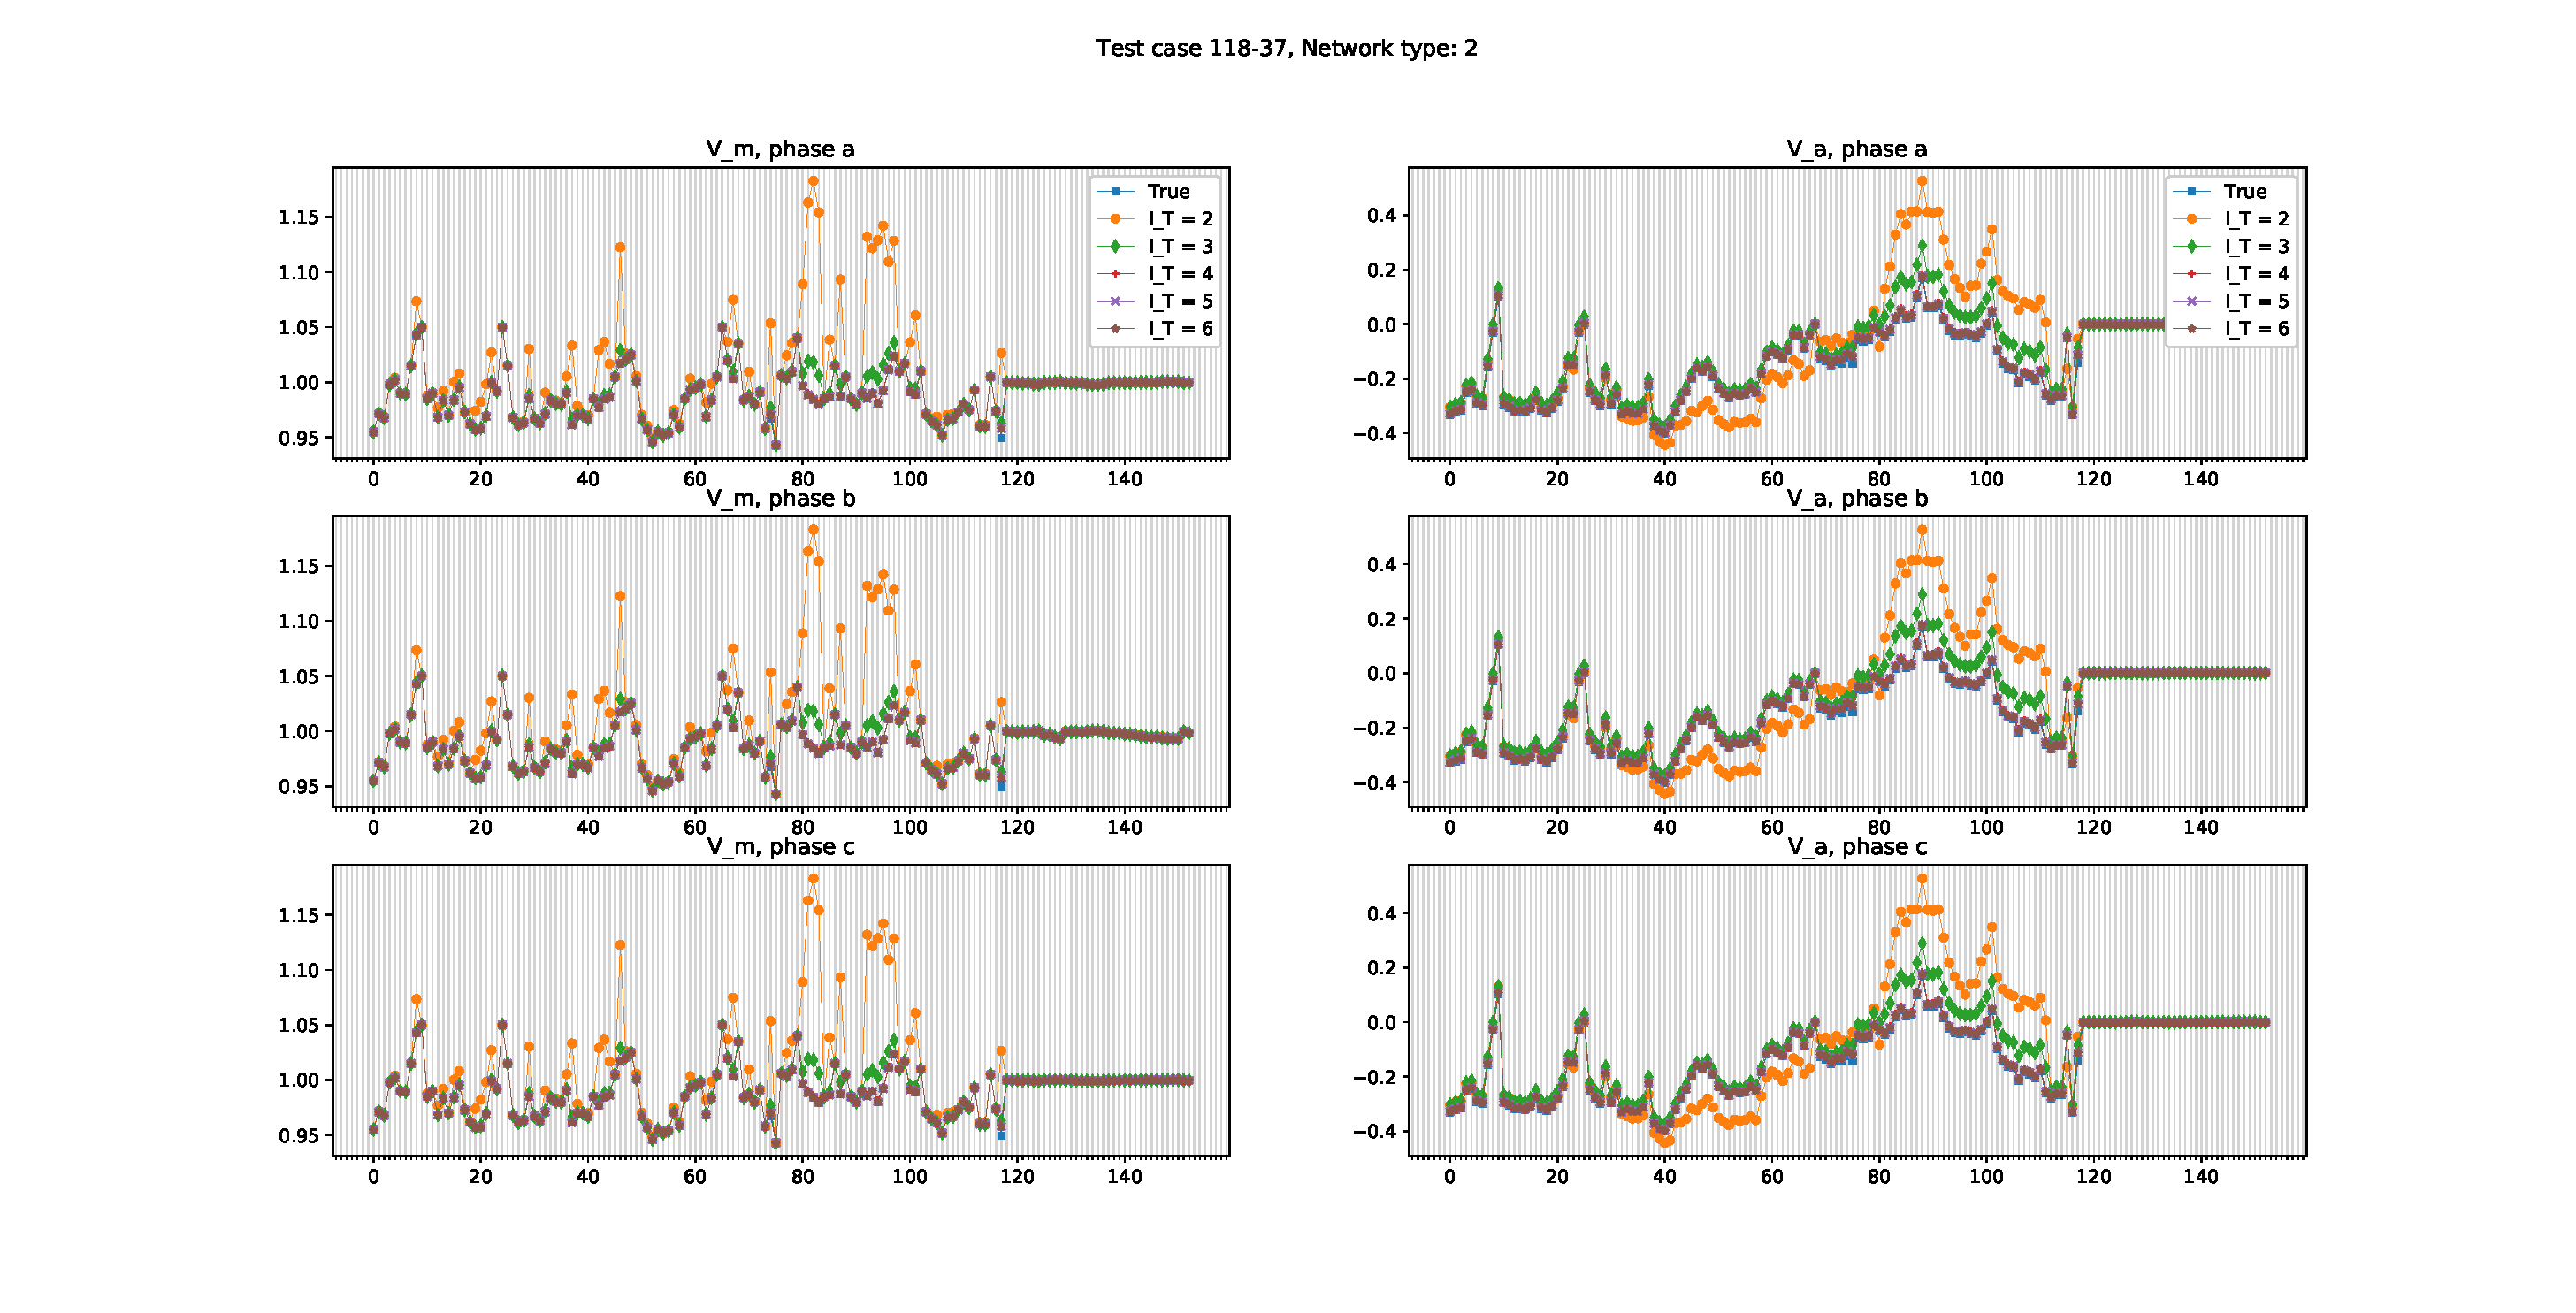
\includegraphics[width=\textwidth]{Images/MAI_N2.eps}
\caption{Voltage profile (left: magnitude, right: angle) of the MAI-schemes with increasing number of subiterations, applied on homogeneous networks}\label{fig:MAIN2}
\end{figure}
\begin{figure}[h]
\centering
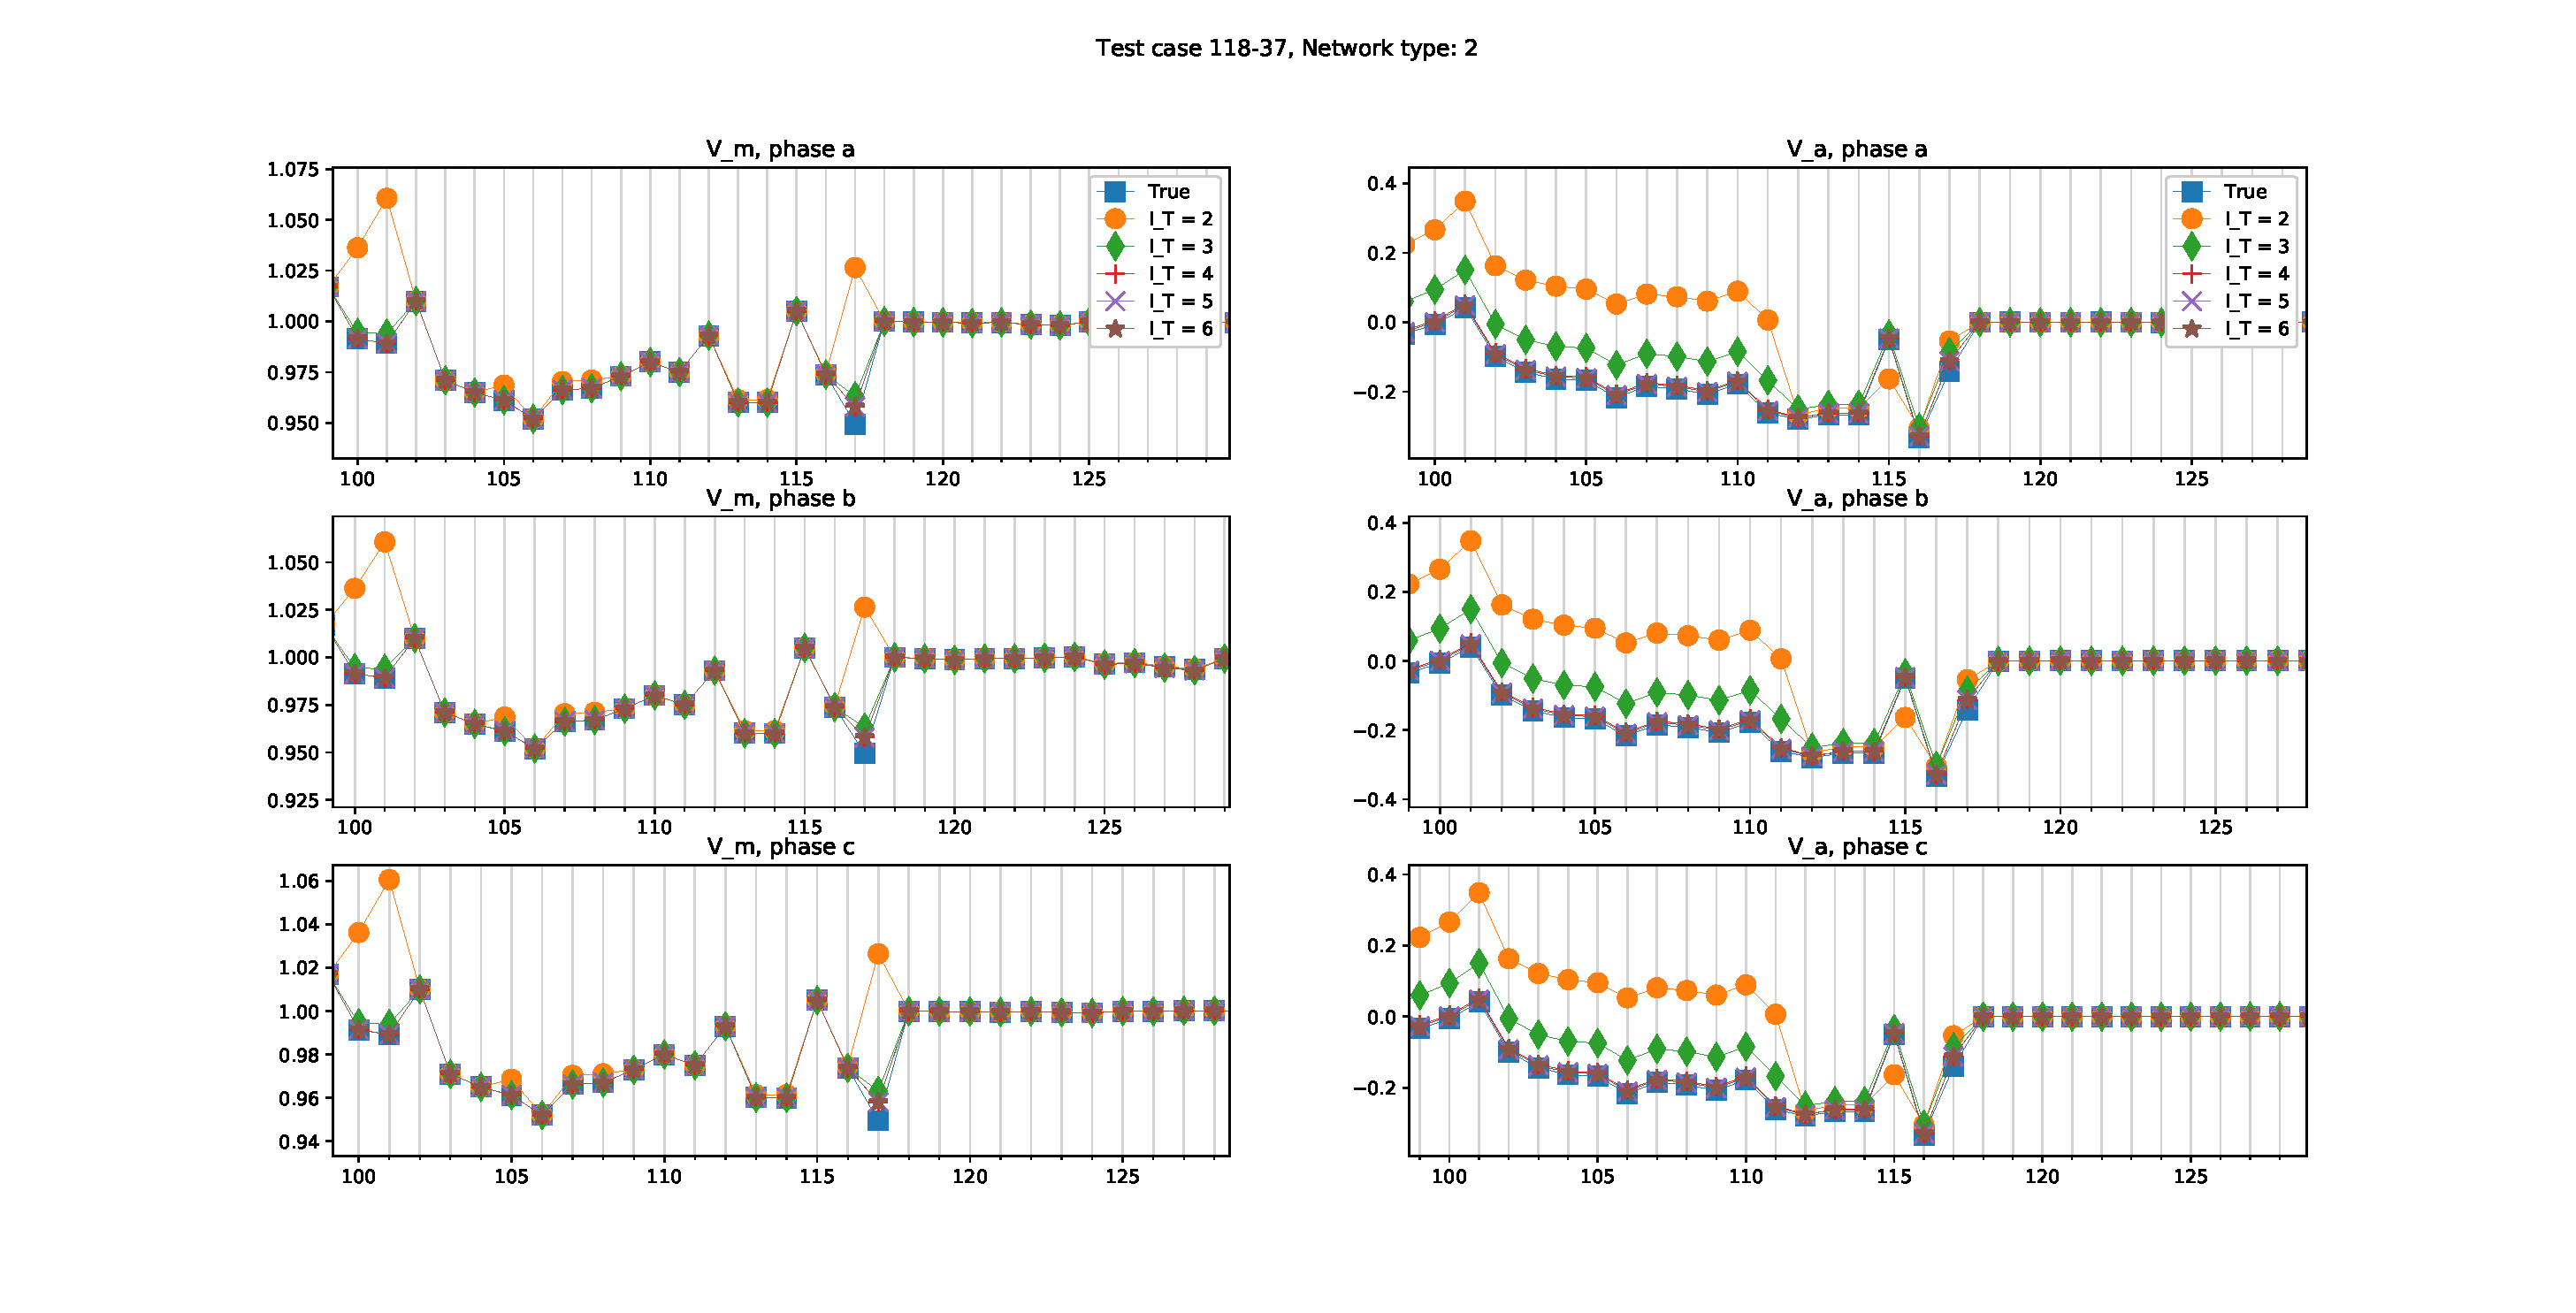
\includegraphics[width=\textwidth]{Images/Z_MAI_N2.eps}
\caption{A magnified version of figure \ref{fig:MAIN2} of the buses surrounding the connection bus.}\label{fig:ZMAIN2}
\end{figure}
\begin{figure}[h]
\centering
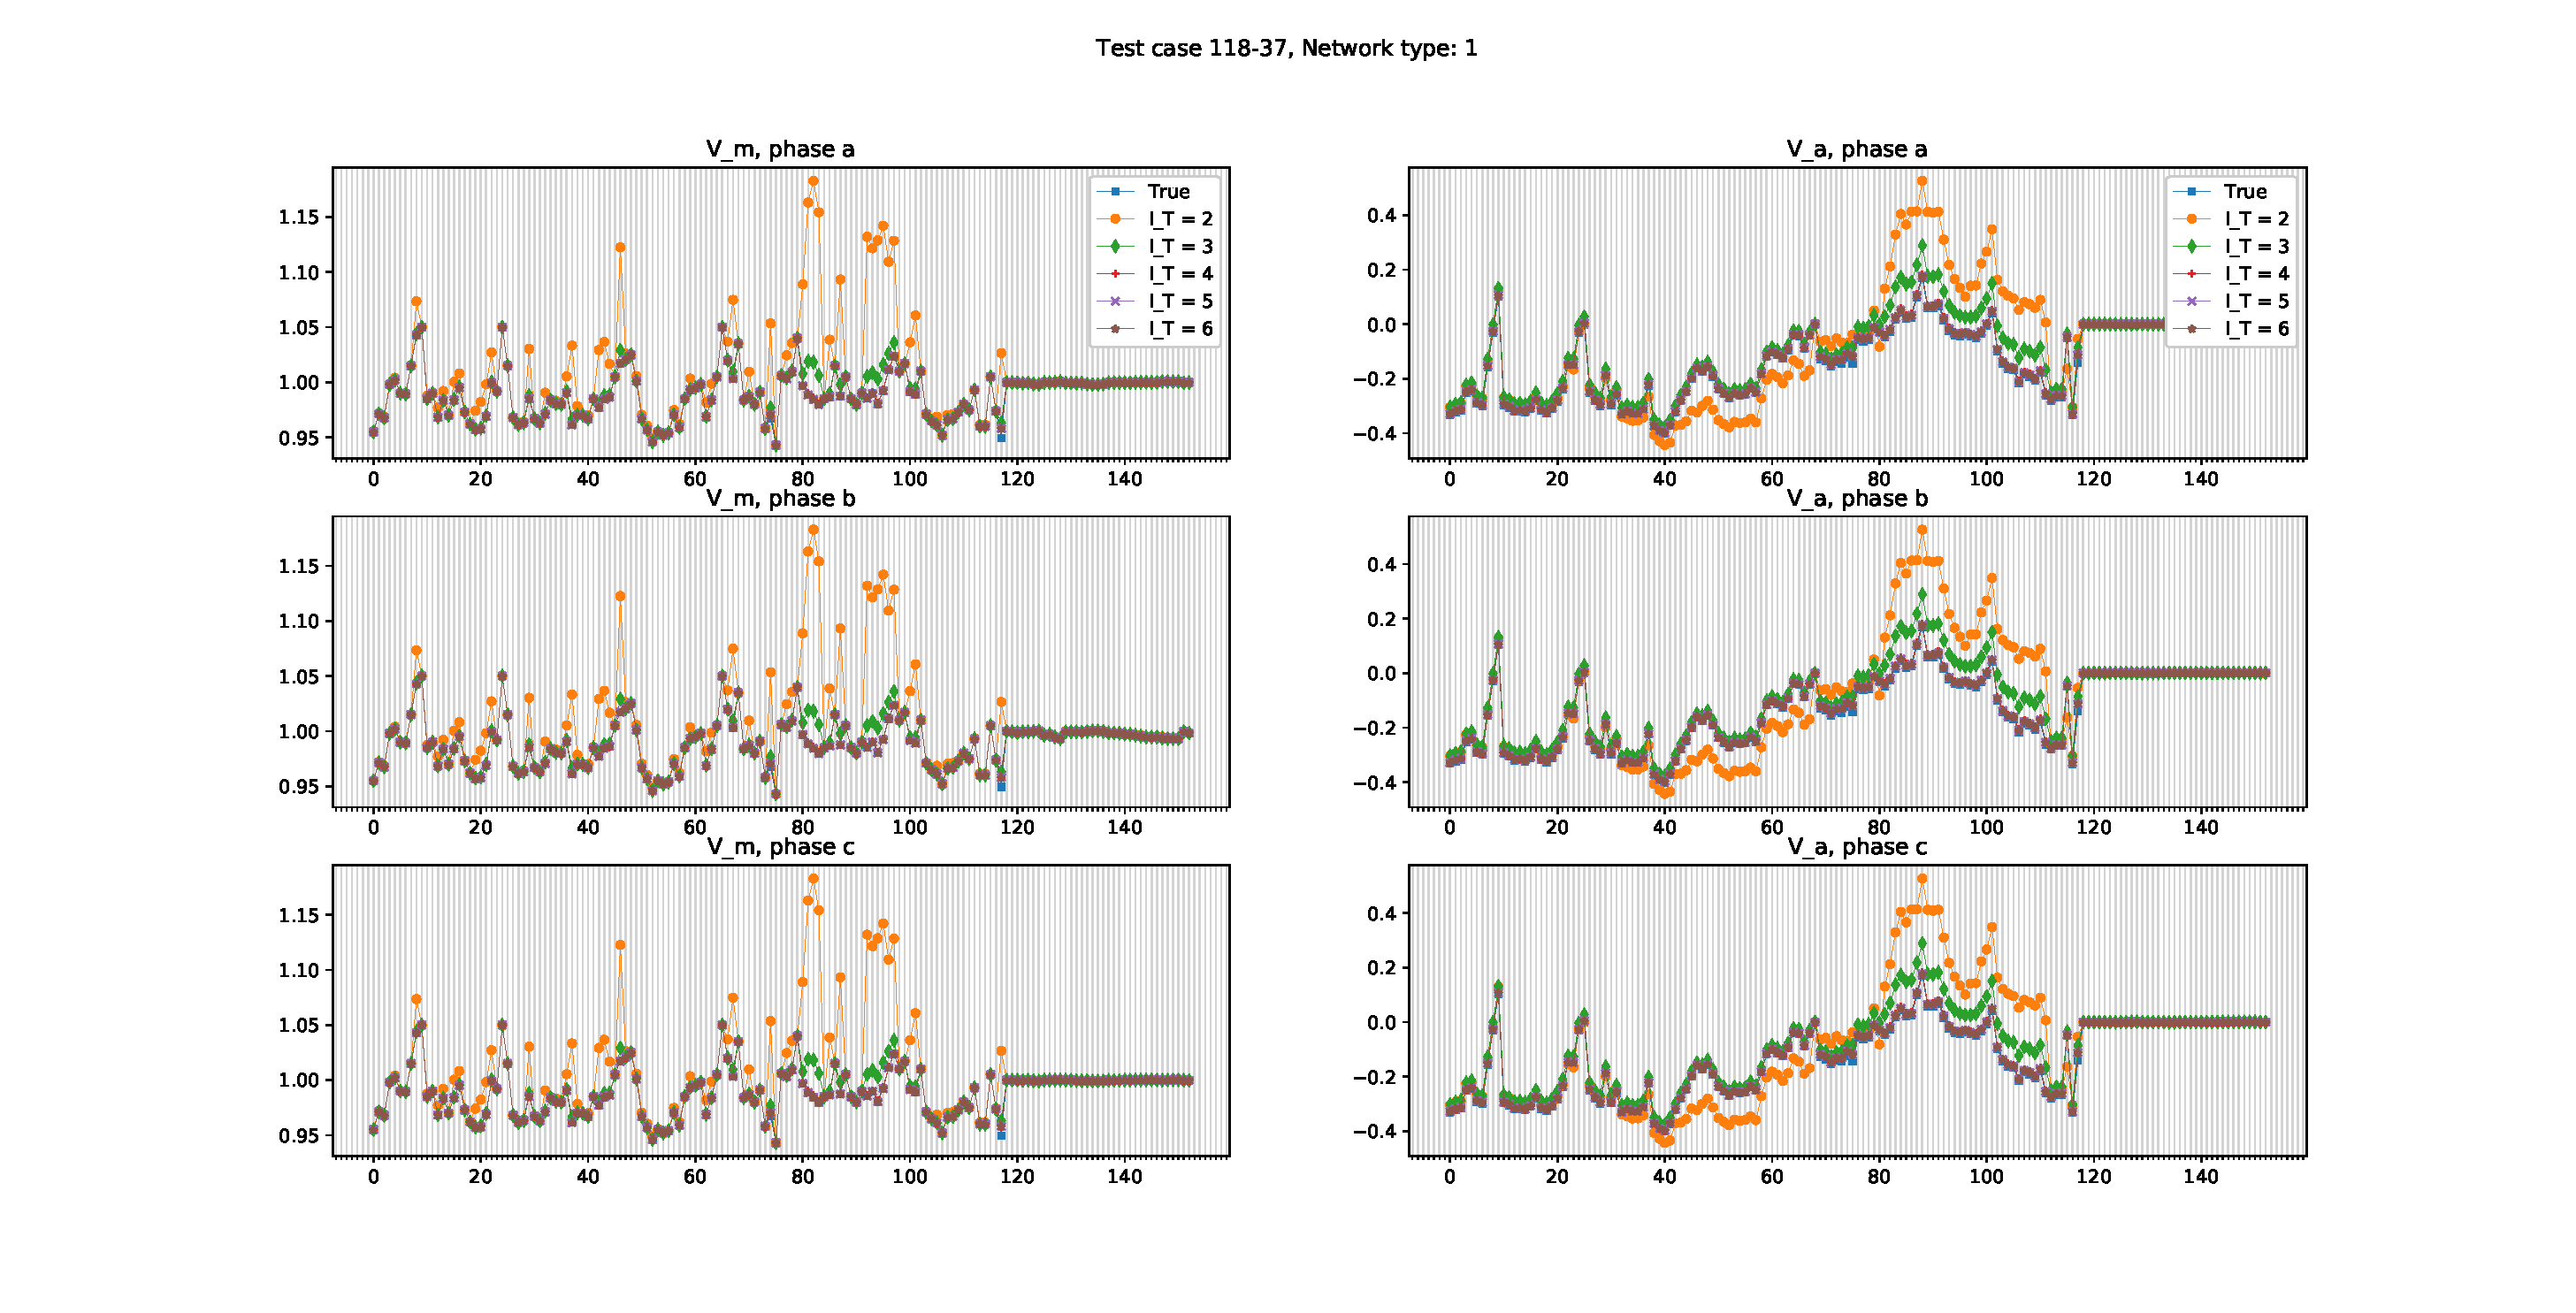
\includegraphics[width=\textwidth]{Images/MAI_N1.eps}
\caption{Voltage profile (left: magnitude, right: angle) of the MAI-schemes with increasing number of subiterations, applied on hybrid networks}\label{fig:MAIN1}
\end{figure}
\begin{figure}[h]
\centering
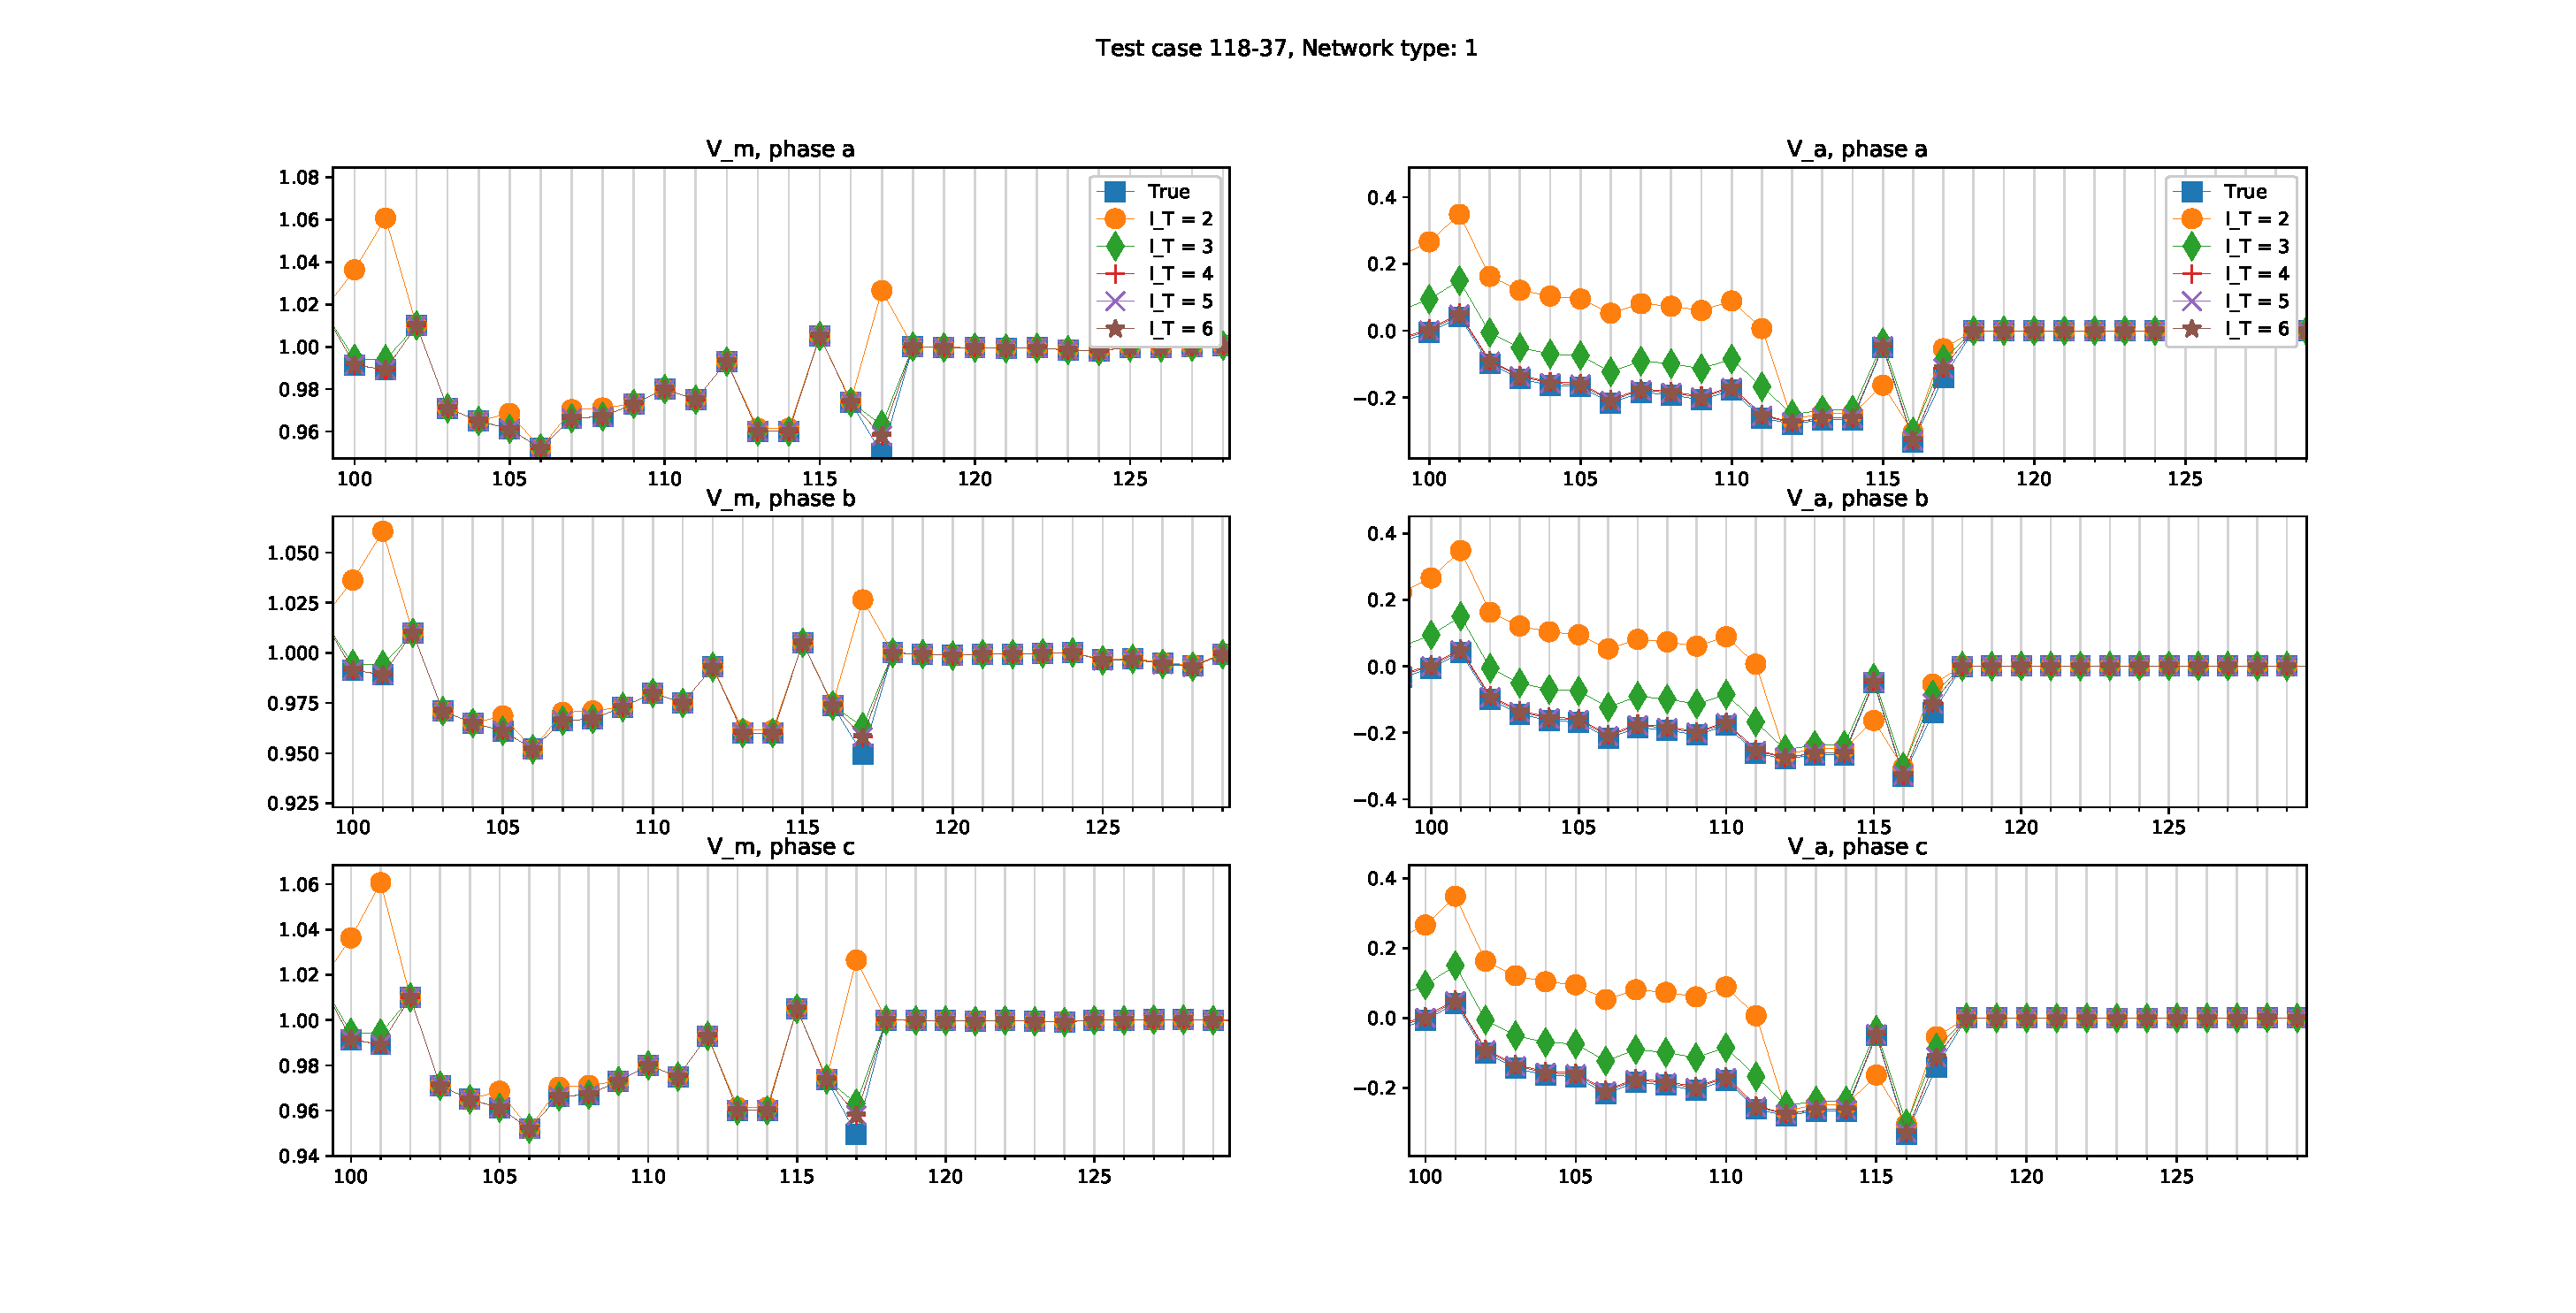
\includegraphics[width=\textwidth]{Images/Z_MAI_N1.eps}
\caption{A magnified version of figure \ref{fig:MAIN1} of the buses surrounding the connection bus.}\label{fig:ZMAIN1}
\end{figure}